\newgeometry{top=2cm, bottom=2cm, left=3cm, right=3cm}
\begin{adjustwidth}{8.5cm}{0cm}
    При  $n=5$ дело обстоит сложнее, так как мы получаем уравнение четвертой степени
    \begin{center}
        $z^{4}+z^{3}+z^{2}+z+1=0$, \quad(3)
    \end{center}
    имеющее четыре корня $\epsilon_{1}, \epsilon_{2}, \epsilon_{3}, \epsilon_{4} $ (рис. б). Чтобы решить его, разделим сначала уравнение (3) на $z^{2}$. Получим
    \begin{center}
        $ z^{2}+\frac{1}{z^{2}}+z+\frac{1}{x}+1=0 $, или \\[1em]$ (z+\frac{1}{z})^{2}+(z+\frac{1}{x})-1=0 $.
    \end{center}
    \vspace{1em}
    \noindent
    Сделаем подстановку $ \omega=z+\frac{1}{z} $:
    \begin{center}
        $ \omega^{2}+\omega-1=0 $.  \quad(4)
    \end{center}
    \noindent
    Отсюда
    \begin{center}
        $ \omega_{1,2}=\frac{1\pm\sqrt{5}}{2} $.
    \end{center}
    \vspace{1em}
    
    Далее, можно найти и $\epsilon{k}$ из уравнений
    \begin{center}
       $ z+\frac{1}{z}=w_{1}, z+\frac{1}{z}=w_{2} $, (5) 
    \end{center}
    \vspace{1em}
    \noindent
    но нам это не нужно; для построения достаточно знать, что $2cos\frac{\pi}{5}$ (удвоенная вещественная часть $\epsilon{1}$) равно
    \begin{center}
        $\epsilon_{1}+\epsilon_{4}=\epsilon_{1}+\frac{1}{\epsilon_{1}}=\omega_{1}=\frac{1+\sqrt{5}}{2}$.
    \end{center}
    \vspace{1em}
    
    Из того, что $\omega_{1}$ - квадратичная иррациональность следует, что $\epsilon_{1}$ и $\epsilon_{4}$ представляют собой квадратичные иррациональности. Для $\epsilon_{2}$ и $\epsilon_{3}$ рассуждаем в точности так же.\par
    
    Итак, для $ n=5 $ решение нашей задачи удалось свести к последовательному решению двух квадратных\\[1em]
    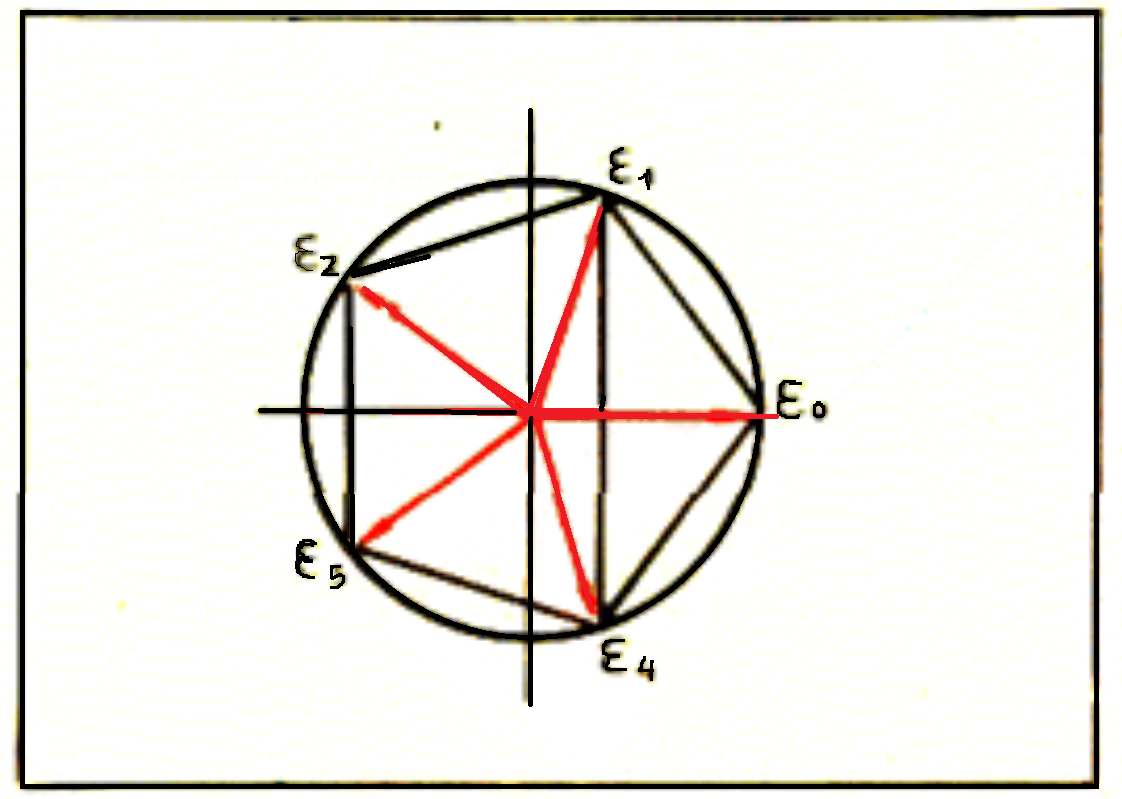
\includegraphics[width=6.5cm]{Untitled1.png}\\
    \scriptsize\textbf{Рис. б.}
    \begin{flushright}
        \small\textbf{5}
    \end{flushright}
\end{adjustwidth}

    


    

